%%%%%%%%%%%%%%%%%%%%%%%%%%%%%%%%%%%%%%%%%%%%%%%%%%%%%%%%%%%%%%%%%%%%%%%%%%
% File: Lecture_1.tex
% Authors: James Kress
% Date: February 1, 2014
% Description: 
%%%%%%%%%%%%%%%%%%%%%%%%%%%%%%%%%%%%%%%%%%%%%%%%%%%%%%%%%%%%%%%%%%%%%%%%%%

%<<<<<<<<<<<<<<<<<<<<<<<<<<<<<<<<<<<<<<<<<<<<<<<<<<<<<<<<<<<<<<<<<<<<<<<<<<<<<%
% Document package information
%>>>>>>>>>>>>>>>>>>>>>>>>>>>>>>>>>>>>>>>>>>>>>>>>>>>>>>>>>>>>>>>>>>>>>>>>>>>>>%
\documentclass[xcolor=dvipsnames]{beamer} 
%%%%%%%%%%%%%%%%%%%%%%%%%%%%%%%%%%%%%%%%%%%%%%%%%%%%%%%%%%%%%%%%%%%%%%%%%%
% File: _TeXdefs.tex
% Author: James Kress
% Date: January 25, 2014
% Description: A tex file containing the \usepackage declarations, and
%			   other document critial style settings.
%%%%%%%%%%%%%%%%%%%%%%%%%%%%%%%%%%%%%%%%%%%%%%%%%%%%%%%%%%%%%%%%%%%%%%%%%%

%-----------Package imports
\usepackage{graphicx}
\usepackage{pgfpages}
\usepackage{tikz}
\usepackage{latexsym}
\usepackage{verbatim}
%//////////END package imports


%----------Style elements
\useoutertheme{infolines} 
\usetheme{Frankfurt} 
\usepackage{../theme/beamercolorthemeoregon}
\setbeamertemplate{sections/subsections in toc}[default]
\setbeamertemplate{footline}
{
\leavevmode%
  \hbox{%
  \begin{beamercolorbox}[wd=.3\paperwidth,ht=2.25ex,dp=.75ex,center]{institute in head/foot}%
    \usebeamerfont{institute in head/foot}\insertshortinstitute
  \end{beamercolorbox}%
    \begin{beamercolorbox}[wd=.4\paperwidth,ht=2.25ex,dp=.75ex,center]{title in head/foot}%
      \usebeamerfont{title in head/foot}\insertshorttitle
    \end{beamercolorbox}%
  \begin{beamercolorbox}[wd=.3\paperwidth,ht=2.25ex,dp=.75ex,center]{date in head/foot}%
    \usebeamerfont{date in head/foot}\insertshortdate\hspace*{3em}
    \insertframenumber{} / \inserttotalframenumber\hspace*{1ex}
  \end{beamercolorbox}}%
  \vskip0pt%
}
%/////////END style elements


%---------Command Declarations
\DeclareGraphicsExtensions{.pdf, .jpeg, .png, .jpg}
\graphicspath{ {../images/} }
\newcommand{\className}{\text{CIS 410/510} \\ \text{Parallel Computing}}
\newcommand{\departmentName}{\textit{Department of Computer and 
									Information Science \\ University of Oregon}}
%/////////END command declarations


%---------Setup pdf properties
\hypersetup{
	pdfusetitle=true,
    bookmarks=true,         	% show bookmarks bar?
    unicode=false,          	% non-Latin characters in Acrobat’s bookmarks
    pdftoolbar=true,        	% show Acrobat’s toolbar?
    pdfmenubar=true,        	% show Acrobat’s menu?
    pdffitwindow=false,     	% window fit to page when opened
    pdfstartview={Fit},   		% fits the width of the page to the window    
    pdfauthor={},     % author
    pdfsubject={Parallel Programming},   	% subject of the document
    pdfcreator={},   			% creator of the document
    pdfproducer={}, 			% producer of the document
    pdfkeywords={University of Oregon, parallel programming}, 
    pdfnewwindow=true,      	% links in new window
    colorlinks=true,       		% false: boxed links; true: colored links
    linkcolor=white,          	% color of internal links
    hidelinks,
    citecolor=green,        	% color of links to bibliography
    filecolor=magenta,      	% color of file links
    urlcolor=cyan,           	% color of external links
    linktoc=page,
    pageanchor = true
}
%//////////END setup pdf properties


%END ALL


%<<<<<<<<<<<<<<<<<<<<<<<<<<<<<<<<<<<<<<<<<<<<<<<<<<<<<<<<<<<<<<<<<<<<<<<<<<<<<%
% END Document package information
%>>>>>>>>>>>>>>>>>>>>>>>>>>>>>>>>>>>>>>>>>>>>>>>>>>>>>>>>>>>>>>>>>>>>>>>>>>>>>%

%=============================================================================%
% Beginning: Title Page Material
%=============================================================================%
\begin{document}
	\title[Map Pattern]{Parallel Control Patterns\\Map}
	\author[]{\className}
	\institute[\className]{\departmentName}
	\date{} 

	\titlegraphic{\centering 
		$\vcenter{\hbox{
\includegraphics[height=.31in,width=2.0in]{oregonLogo}}}$
	}

	\begin{frame}
		\maketitle
	\end{frame}
%-----------------------------------------------------------------------------%
% End: Title Page Material
%-----------------------------------------------------------------------------%


%=============================================================================%
% Section -> Map
%=============================================================================%
\section{Map} 

	\begin{frame} \frametitle{Table of Contents}
		\tableofcontents[currentsection]
	\end{frame} 
	
	
	\subsection*{Mapping}
		\begin{frame}[fragile] \frametitle{Mapping}
			\begin{itemize}
					\item ``Do the same thing many times"
					\item \begin{verbatim}
					foreach foo in Foo:
					    do something
					\end{verbatim}
					\item Well-known higher order function in languages like ML, 
					Haskell, Scala
					\[ \texttt{map} : \forall a b. (a \to b) \to \texttt{List}\langle 
					a\rangle \to \texttt{List}\langle b\rangle \]
					applies a function to each element in a list and returns a list 
	                of results.\\
			\end{itemize}
		\end{frame}
			
		\begin{frame} \frametitle{Example Maps}
			\begin{itemize}
				\item Add $1$ to every item in an array
				\item Double every item in an array
				\item Convert a list of temperatures from Celsius to Fahrenheit
				\item 3D animation: render each frame in a sequence
				\item For each point on the complex plane, compute if in Mandelbrot 
				set
			\end{itemize}
			\begin{columns}
	  			\begin{column}{0.4\textwidth}
					\begin{block}{Famous Fractal}
						Point $c$ if the sequence $z_{n+1} = z_n^2 + c$ starting at
						zero is bounded
					\end{block}
			    \end{column}
			    \begin{column}{0.6\textwidth}
					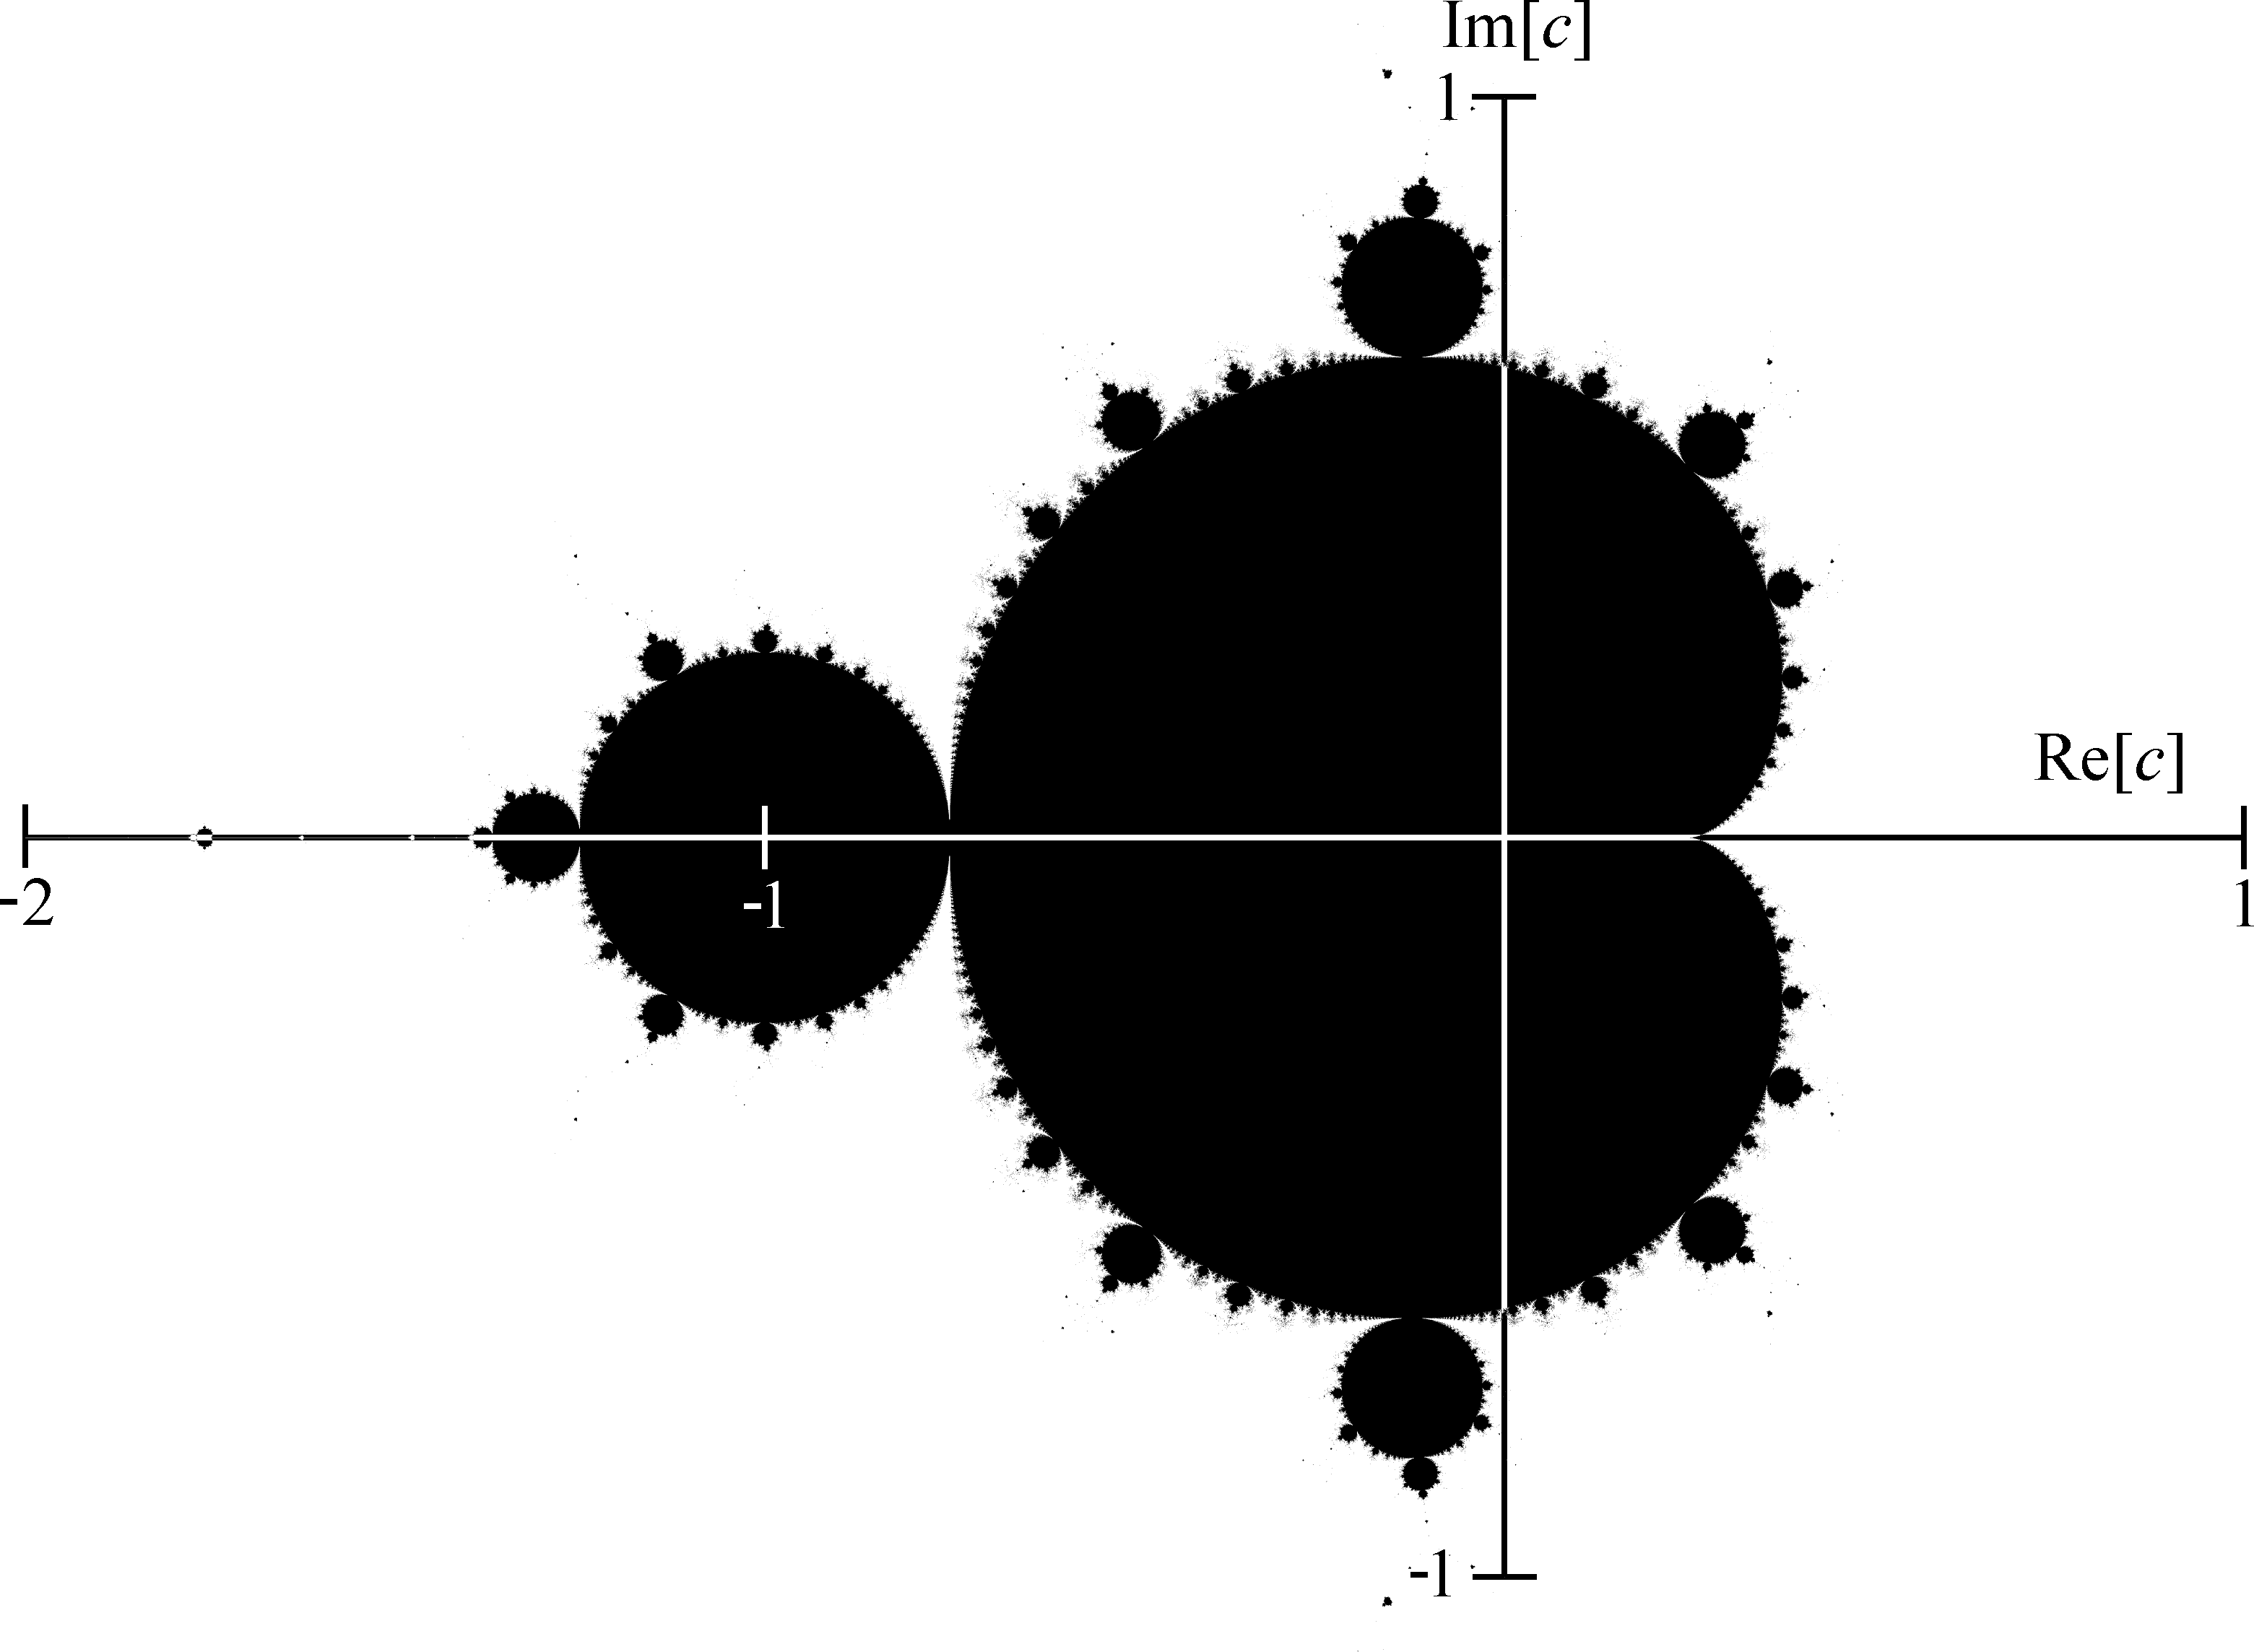
\includegraphics[width=60mm]{Images/Mandelset_hires.png}
				\end{column}
			\end{columns}
		\end{frame}
			
		\begin{frame} \frametitle{Example Maps Cont.}
			Some things might not look like maps at first...but can often be 
			implemented as map+some pre and/or post processing
			\begin{itemize}
			    \item Password Cracking
			    \item Bitcoin Mining
			    \item Procedural Terrain Generation 
			    \item Number Theoretic Problems (e.g. Quadratic Field Sieve
                used in fast factoring)
			    \item Parameter Estimation for Scientific Models
			\end{itemize}
			\begin{alertblock}{Not just arrays}
				Map pattern is datatype independent.  With various levels of 
				efficiency we can map over lists, trees, graphs, etc... Even 
				abstract ``collection" like sequences of numbers
			\end{alertblock}
		\end{frame}
			
		\begin{frame} \frametitle{Key idea}
			\begin{itemize}
				\item map is a ``foreach loop" \pause 
				\alert{where each iteration is independent} \pause
			\end{itemize}
			\begin{block}{Embarrassingly Parallel}
			Independence is big win.  We can run map completely in parallel.
			Significant speedups:\\More precisely: $T(\infty)$ is  $O(1)$ plus
			implementation overhead that is $O(\log{n})$\ldots so $T(\infty)
			\in O(\log n)$\\$T(1) \in O(n)$
			\end{block}
		\end{frame}
			
		\begin{frame}[fragile] \frametitle{Sequential Map}
			\begin{columns}
				\begin{column}{0.5\textwidth}
					\begin{verbatim}
					for(int n = 0;
						   n < array.length;
						   ++n){
						        process(array[n]);
					}
					\end{verbatim}
			    \end{column}
	  			\begin{column}{0.5\textwidth}
					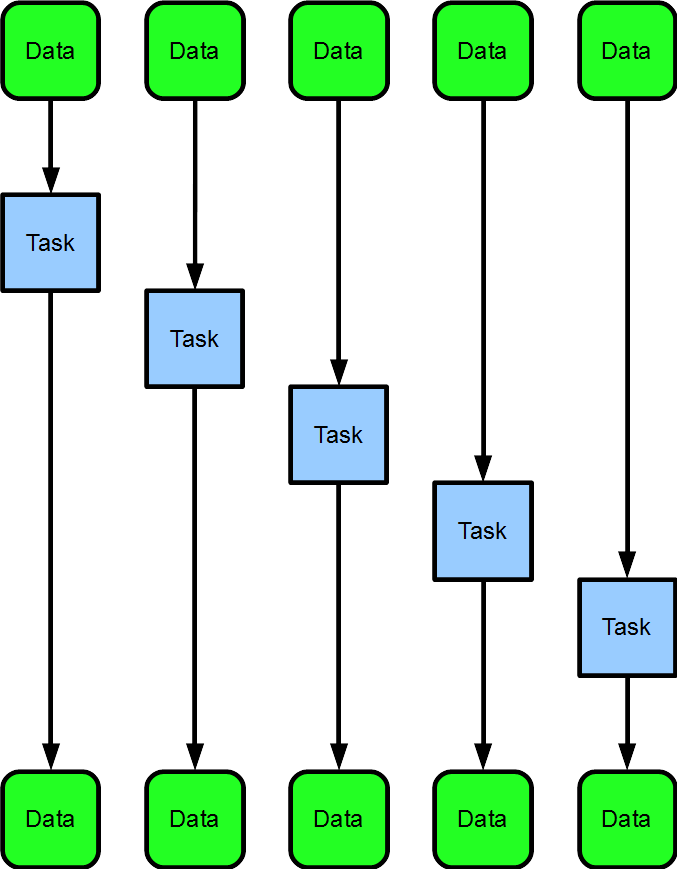
\includegraphics[width=60mm]{images/map_serial.png}
			    \end{column}
			\end{columns}
		\end{frame}
			
			
		\begin{frame}[fragile] \frametitle{Parallel Map}
			\begin{columns}
				\begin{column}{0.5\textwidth}
					\begin{verbatim}
					parallel_for_each(
					    x in array){
						        process(x);
					}
					\end{verbatim}
			    \end{column}
		  		\begin{column}{0.5\textwidth}
					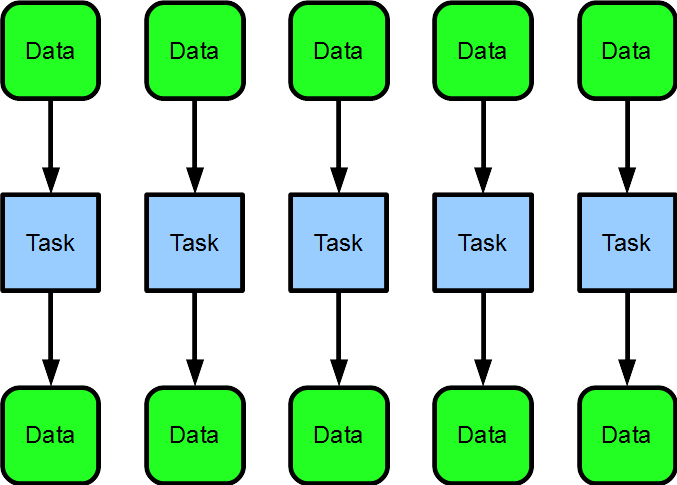
\includegraphics[width=60mm]{images/map_parallel.png}
				\end{column}
			\end{columns}
		\end{frame}
			
		\begin{frame}[fragile] \frametitle{Comparing Maps}
			\begin{columns}
				\begin{column}{0.5\textwidth}
					\centering{Serial Map}
					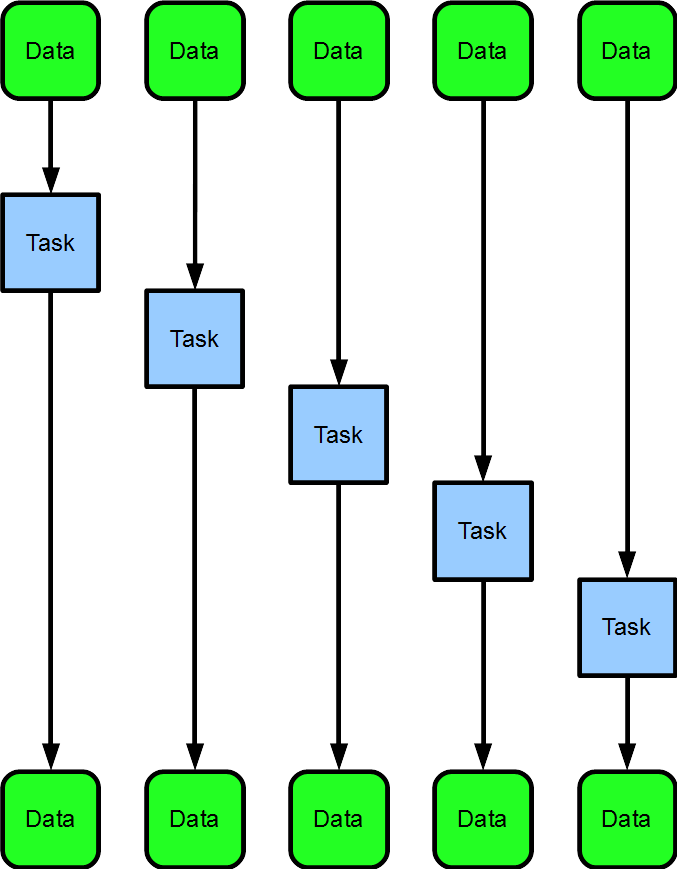
\includegraphics[width=55mm]{images/map_serial.png}
			    \end{column}
	  			\begin{column}{0.5\textwidth}
	  				\centering{Parallel Map}
					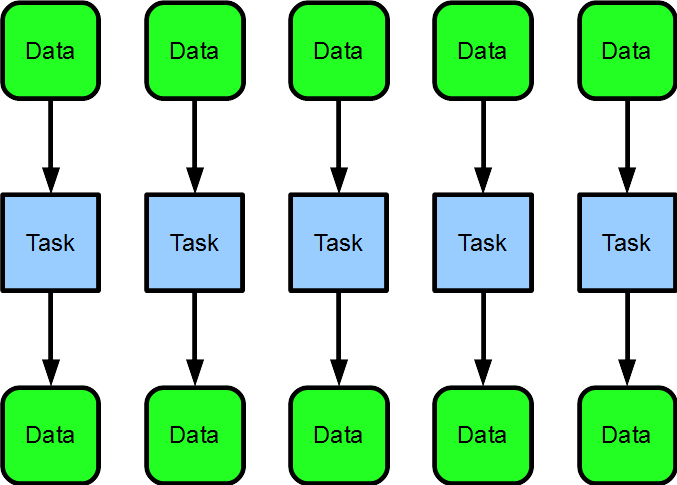
\includegraphics[width=55mm]{images/map_parallel.png}\pause
					\begin{block}{Speedup}
						This space here is \textbf{speedup}. With the parallel
                        map, our program finished execution early, while the 
                        serial map is still running.
					\end{block}
			     \end{column}
			\end{columns}
		\end{frame}
			
		\begin{frame} \frametitle{Independence}
			The key to (embarrassing) parallelism is independence.\pause
			\begin{alertblock}{Warning: No shared state!}
				Map function should be ``pure" (or ``pure-ish") and should not 
	            modify shared states.
			\end{alertblock}
			Modifying shared state breaks perfect independence.\\Accidentally
			violating independence may result in non-determinism, data-races, 
			undefined behavior, segfaults, etc. \pause The C/C++ standard has 
			``catch fire semantics" for data races. That means it is part of the 
			programming language semantics for your computer to \textbf{literally
			catch fire} or do absolutely anything.
		\end{frame}
			
		\begin{frame}[fragile] \frametitle{Implementation and API}
			\begin{itemize}
				\item In OpenMP and CilkPlus we have a parallel \texttt{for} 
				language construct
				\item map is a mode of use of parallel \texttt{for}
				\item TBB uses \textbf{higher order functions} with lambda
				expressions/``functors"
				\item Some language (CilkPlus, Matlab, Fortran) provide
				\textbf{array notation} which makes some maps more concise\\
				\begin{exampleblock}{Array Notation}
					\begin{verbatim}
					a[:] = a[:]*5;
					\end{verbatim}
					is CilkPlus array notation for ``multiply every element in 
	                \texttt{a} by $5$" 
				\end{exampleblock}
			\end{itemize}
		\end{frame}
			
		\begin{frame} \frametitle{Generalization?}
			\begin{block}{unary maps}
				So far we have only dealt with mapping over a single collection
			\end{block}
		\end{frame}
			
		\begin{frame} \frametitle{1 to 1 map}
			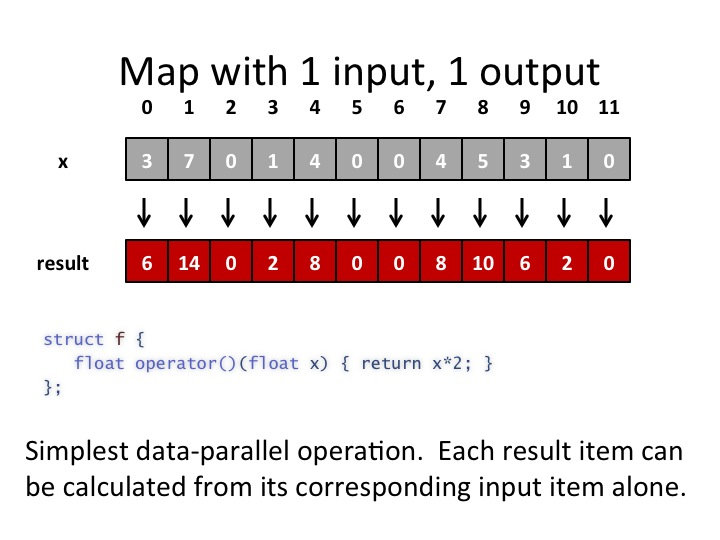
\includegraphics[width=110mm]{images/map1to1.jpg}
		\end{frame}  
			
		\begin{frame} \frametitle{Generalization?}
			\begin{block}{n-ary maps}
				But sometimes it makes sense to map over multiple collections at 
	            once 
			\end{block}
			functional programming languages call this \texttt{zipWith} or 
			sometimes \texttt{map2}
		\end{frame}
			
		\begin{frame} \frametitle{2 to 1 map}
			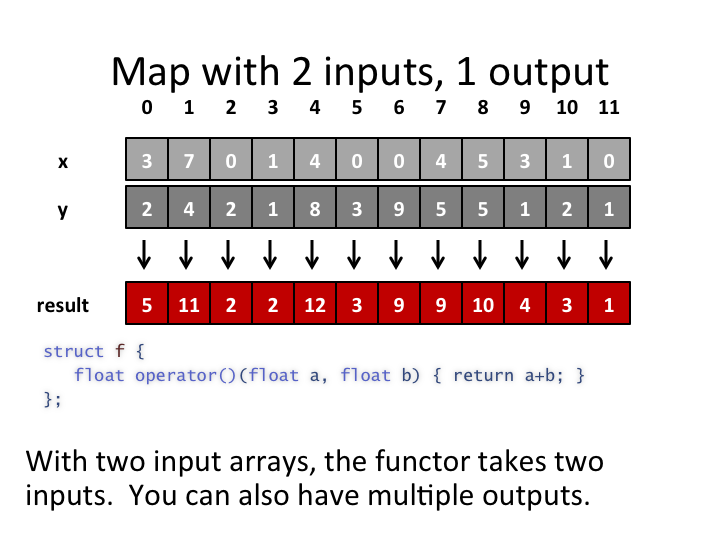
\includegraphics[width=110mm]{images/map2to1.png}
		\end{frame} 
%-----------------------------------------------------------------------------%
% End: Map
%-----------------------------------------------------------------------------%


%=============================================================================%
% Section -> SAXPY Example
%=============================================================================%
\section{Scaled Vector Addition (SAXPY) Example} 

	\begin{frame} \frametitle{Table of Contents}
		\tableofcontents[currentsection]
	\end{frame} 
	
	\subsection{Problem Description}
		\begin{frame} \frametitle{Problem Description}
            \begin{itemize}
                \item $y \leftarrow ax + y$
                    \begin{itemize}
                        \item Scales vector $x$ by $a$ and adds it to vector 
                        $y$ 
                        \item Result is stored in input vector $y$
                    \end{itemize}
                \item SAXPY comes from the BLAS (Basic Linear Algebra 
                Subprograms) library
                \item SAXPY has a low arithmetic intensity, so it does not 
                scale well
            \end{itemize}
		\end{frame}
	
	\subsection{SAXPY Implementations}
		\begin{frame} \frametitle{Serial SAXPY Implementation}
			\begin{figure}
				\centering
				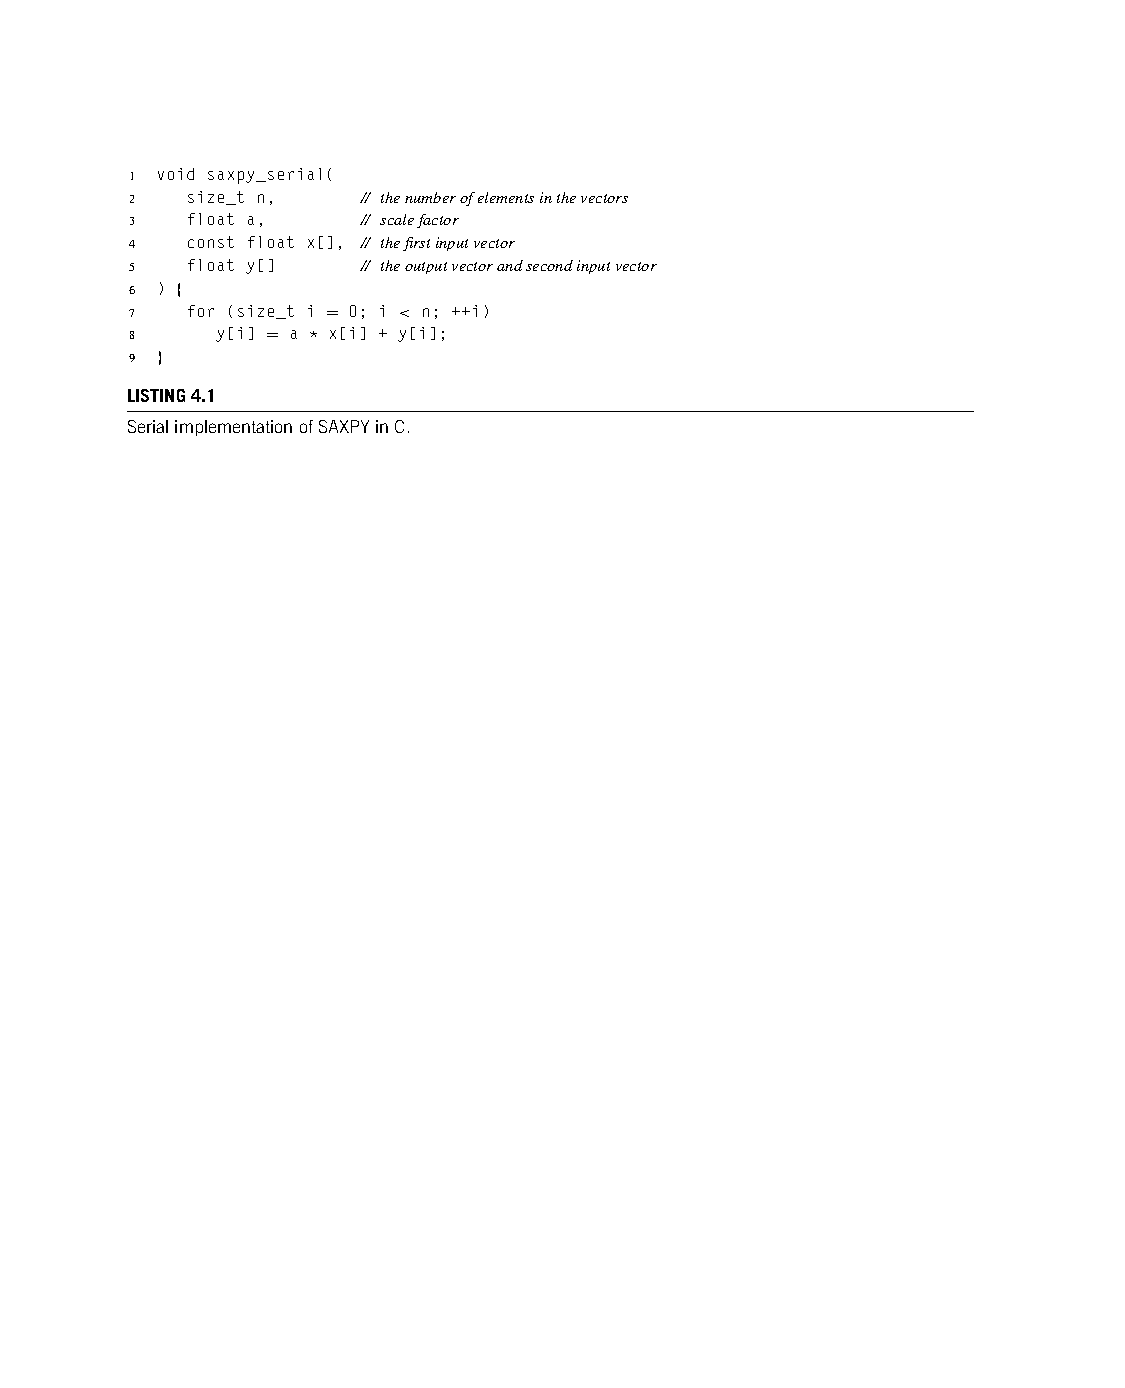
\includegraphics[width=115mm]{images/listing-4-1.pdf}
			\end{figure}
		\end{frame}
		
		\begin{frame} \frametitle{TBB SAXPY Implementation}
			\begin{figure}
				\centering
				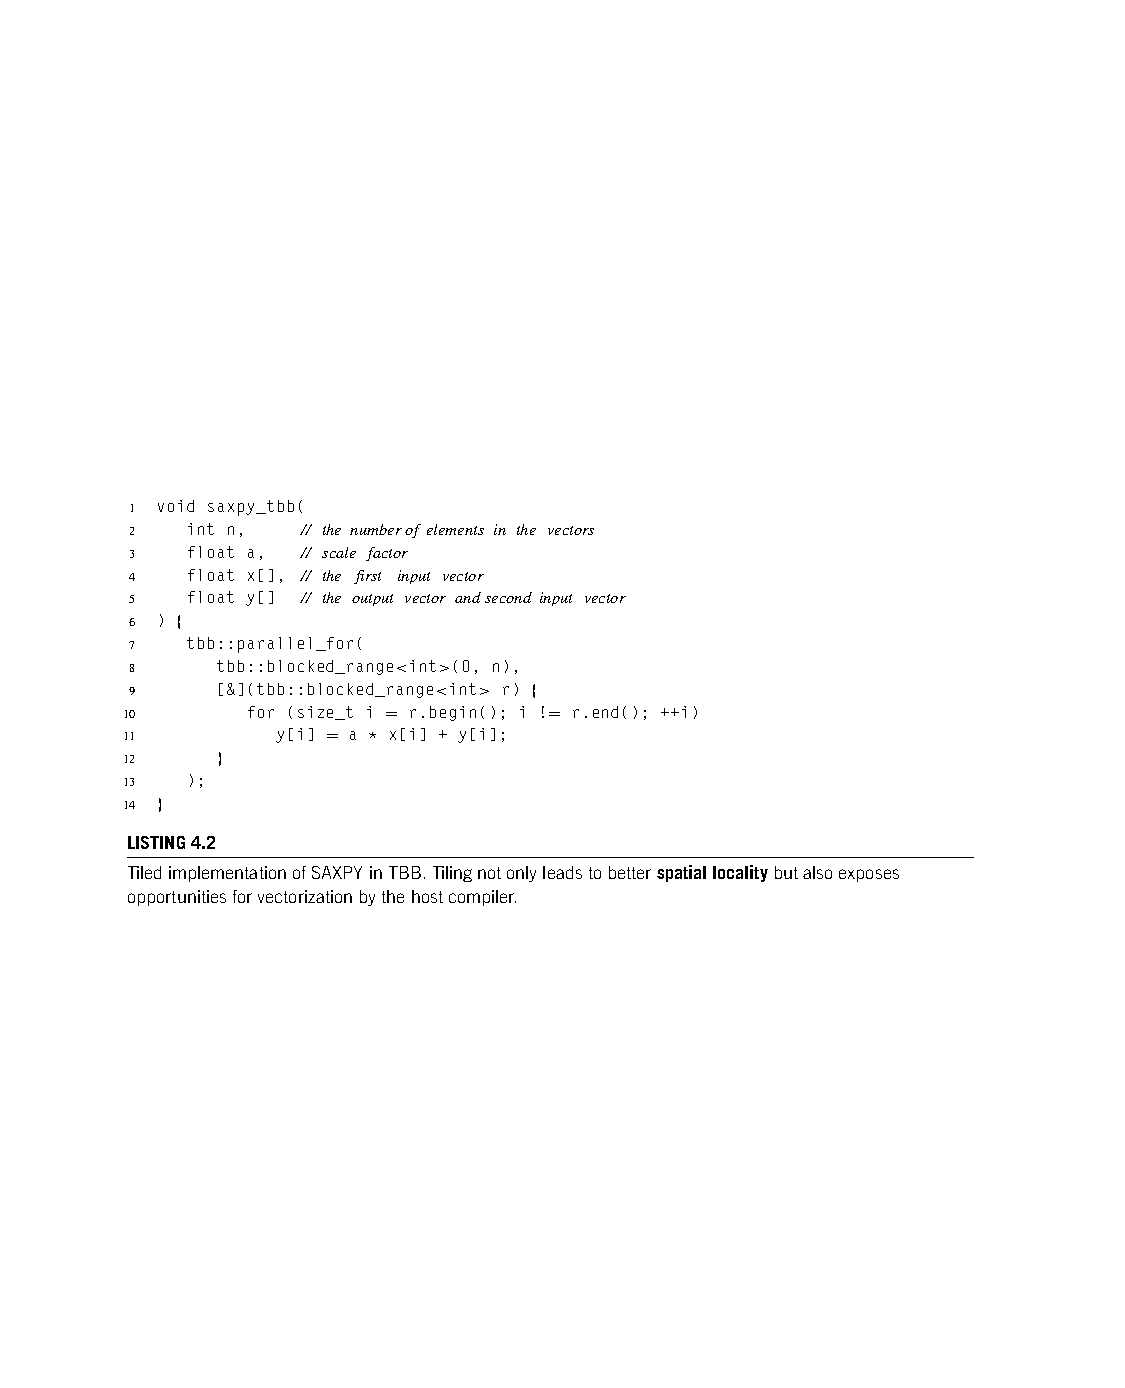
\includegraphics[width=115mm]{images/listing-4-2.pdf}
			\end{figure}
		\end{frame}
		
		\begin{frame} \frametitle{Cilk Plus SAXPY Implementation}
			\begin{figure}
				\centering
				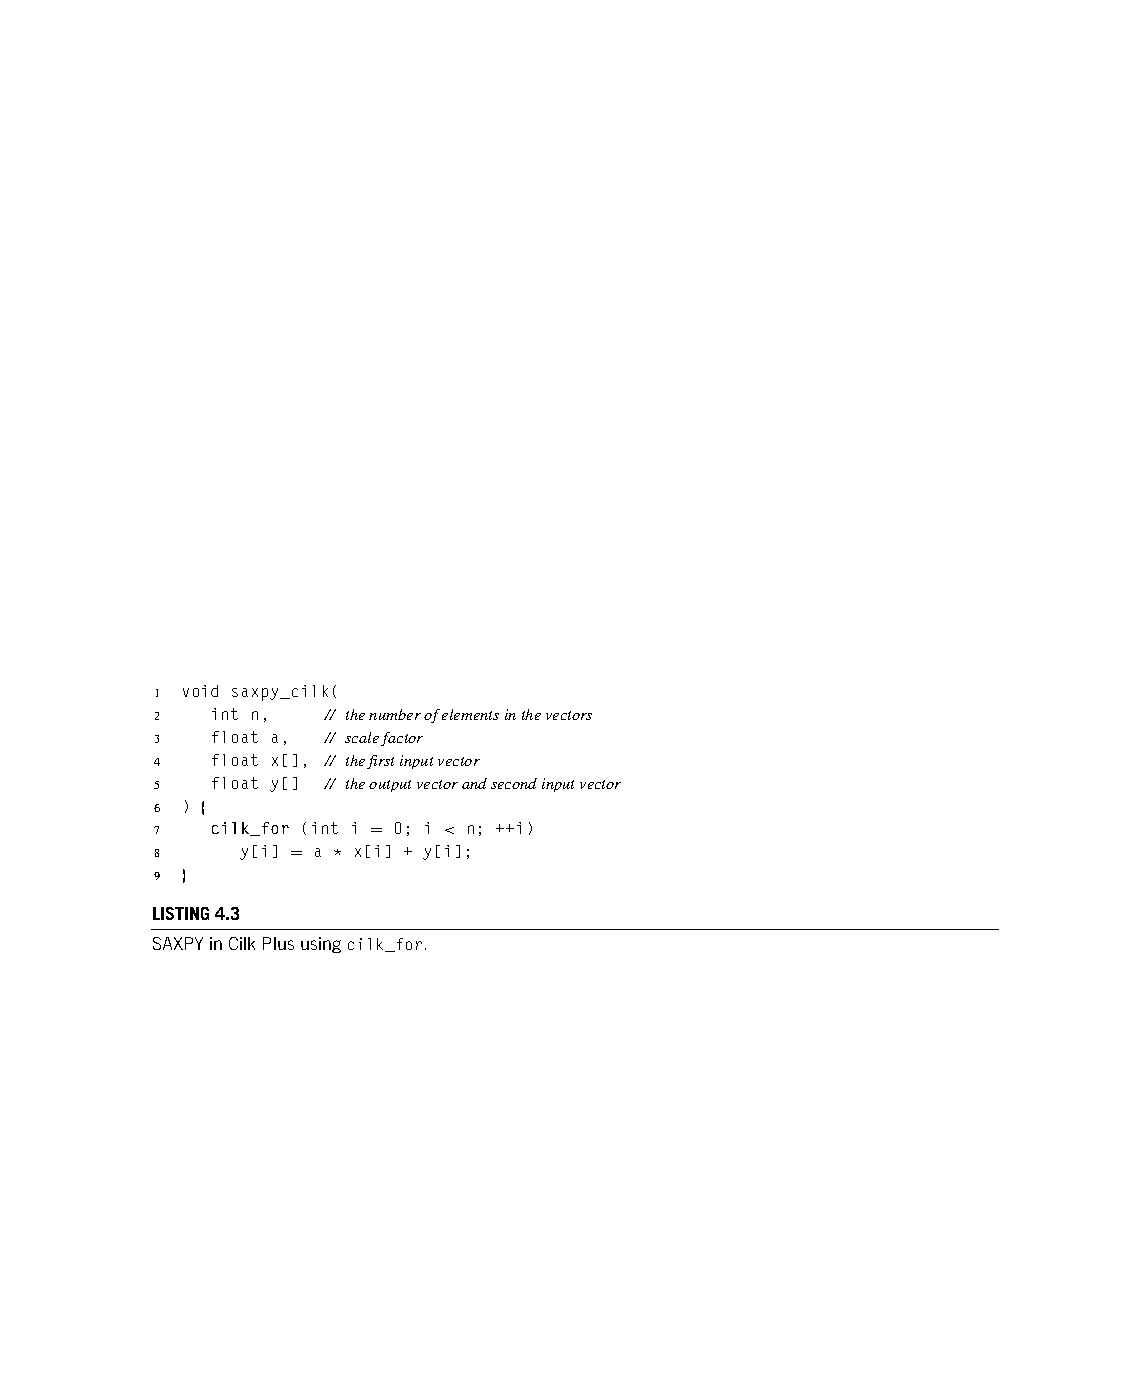
\includegraphics[width=115mm]{images/listing-4-3.pdf}
			\end{figure}
		\end{frame}
		
		\begin{frame} \frametitle{OpenMP SAXPY Implementation}
			\begin{figure}
				\centering
				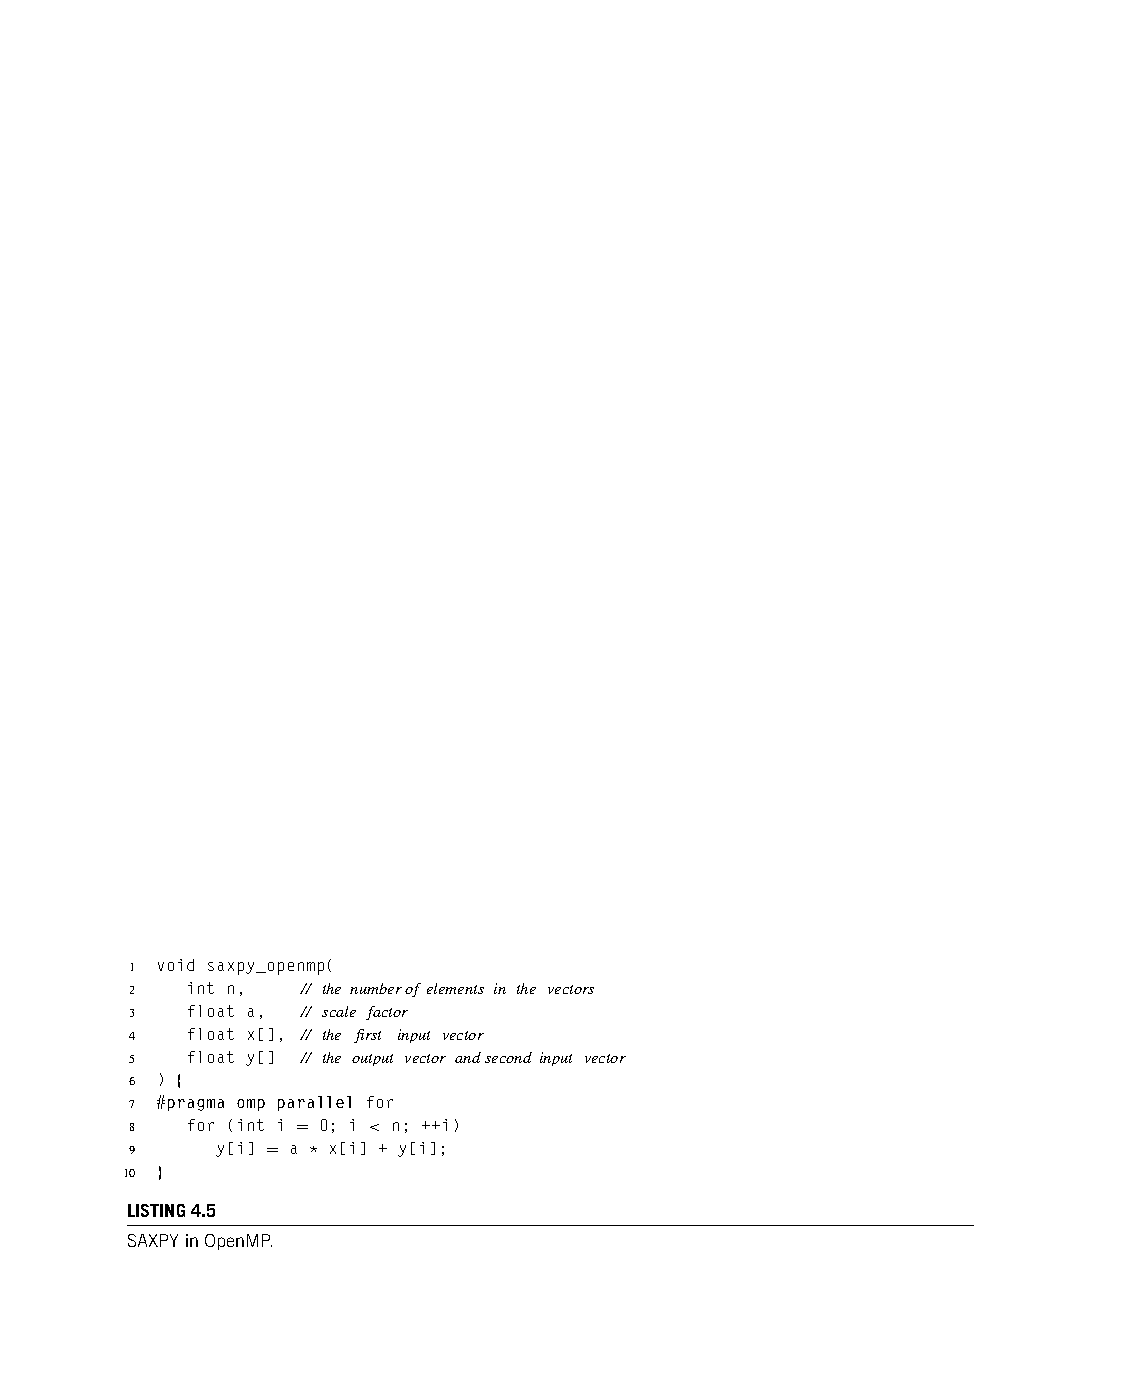
\includegraphics[width=115mm]{images/listing-4-5.pdf}
			\end{figure}
		\end{frame}
%-----------------------------------------------------------------------------%
% End: SAXPY Example
%-----------------------------------------------------------------------------%


%=============================================================================%
% Section -> Optimizations 
%=============================================================================%
\section{Optimizations} 

	\begin{frame} \frametitle{Table of Contents}
		%\tableofcontents
		%\tableofcontents[pausesections]
		\tableofcontents[currentsection]
	\end{frame} 
	
	\subsection{Sequences of Maps}
		\begin{frame} \frametitle{Sequences of Maps}
      		\begin{columns}
        		\begin{column}{0.48\textwidth}
          			\begin{itemize}
            			\item Often several map operations occur in sequence
							\begin{itemize}
	                			\item Vector math consists of many small 
                                operations such as additions and 
                                multiplications applied as maps
	              			\end{itemize}
            			\item A na\"\i ve implementation may write each 
                        intermediate result to memory, wasting memory 
                        bandwidth and likely overwhelming the cache.
          			\end{itemize}
        		\end{column}
        		\begin{column}{0.48\textwidth}
			        \centering
			        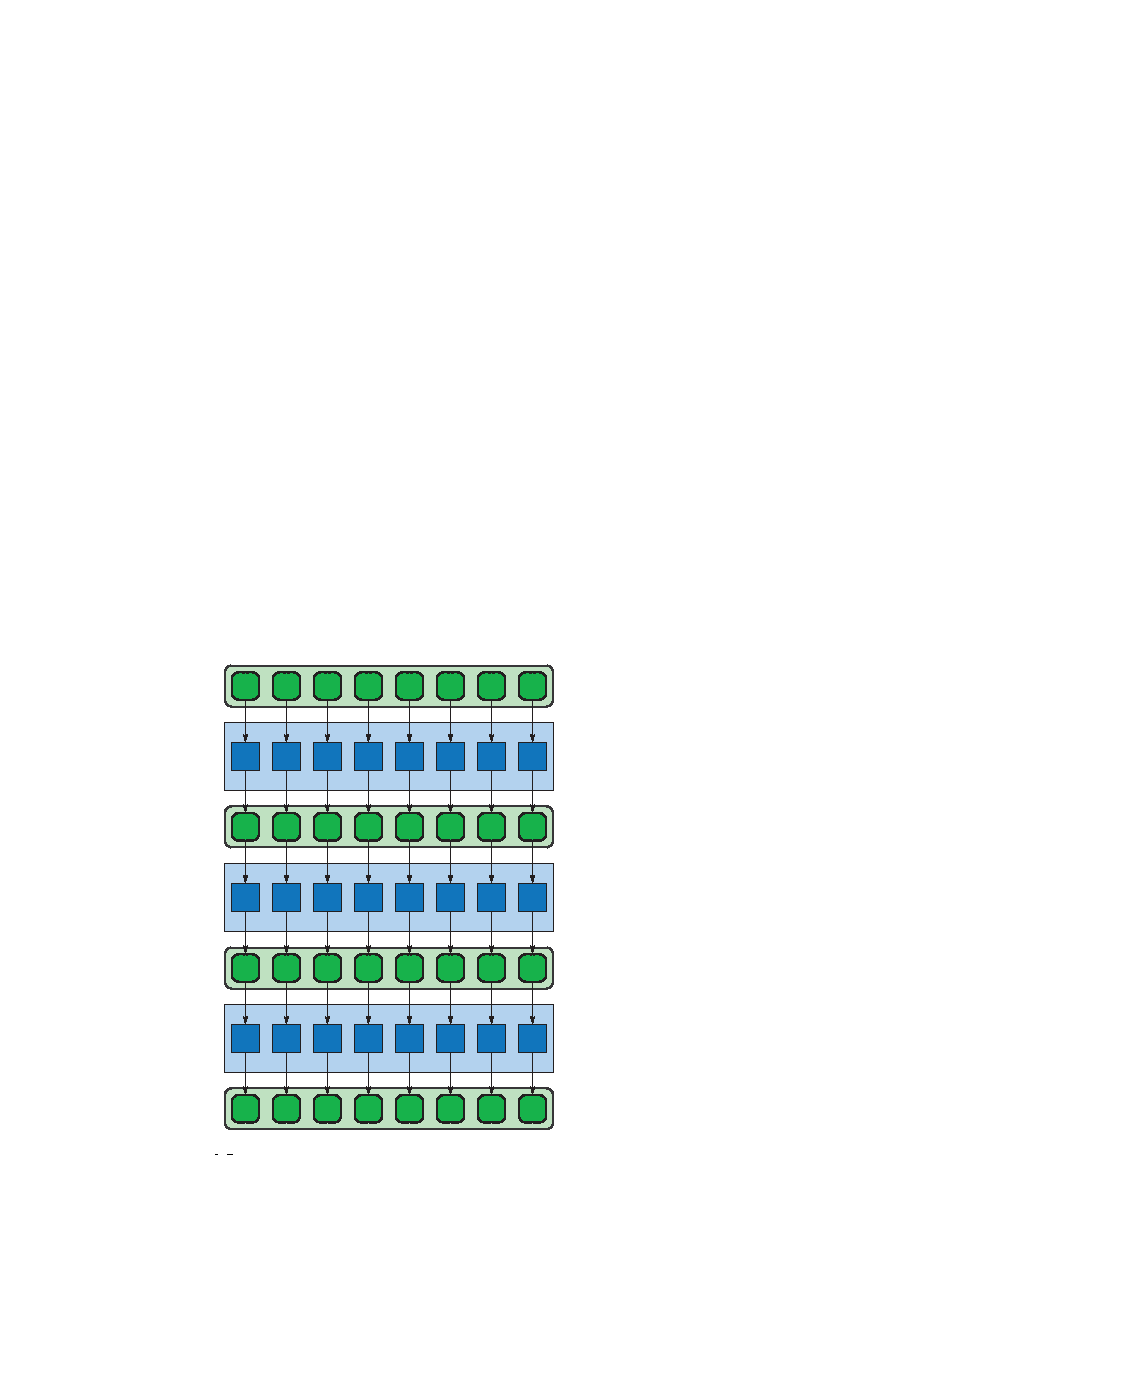
\includegraphics[width=0.9\textwidth]{images/figure-4-2-1}
		        \end{column}
			\end{columns}
		\end{frame}

	\subsection{Code Fusion}
		\begin{frame} \frametitle{Code Fusion}
			\begin{columns}
        		\begin{column}{0.48\textwidth}
          			\begin{itemize}
            			\item Can sometimes ``fuse'' together the operations 
                        to perform them at once
            			\item Adds arithmetic intensity, reduces memory/cache 
                        usage
            			\item Ideally, operations can be performed using 
                        registers alone
          			\end{itemize}
        		\end{column}
        	\begin{column}{0.48\textwidth}
	        	\centering
		        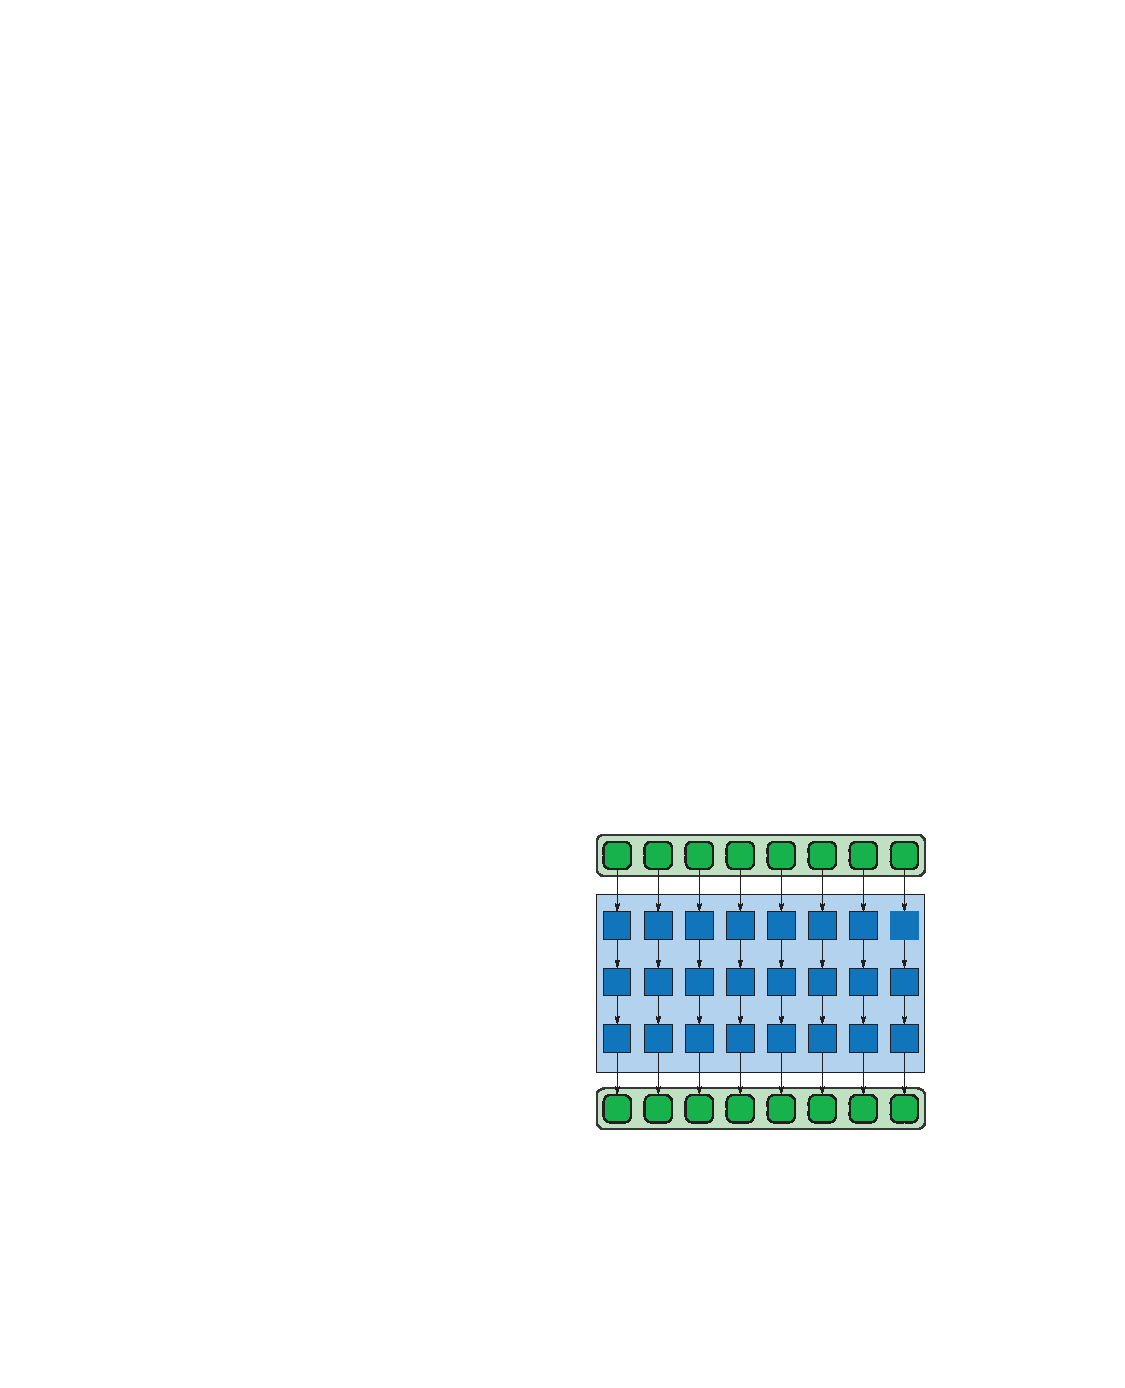
\includegraphics[width=0.9\textwidth]{images/figure-4-2-2}
            \end{column}
           \end{columns}
		\end{frame}

	\subsection{Cache Fusion}
		\begin{frame} \frametitle{Cache Fusion}
			\begin{columns}
        		\begin{column}{0.48\textwidth}
          			\begin{itemize}
            			\item Sometimes impractical to fuse together the map 
                        operations
            			\item Can instead break the work into blocks, giving 
                        each CPU one block at a time
            			\item Hopefully, operations use cache alone
          			\end{itemize}
        		\end{column}
	        	\begin{column}{0.48\textwidth}
	          		\centering
	          		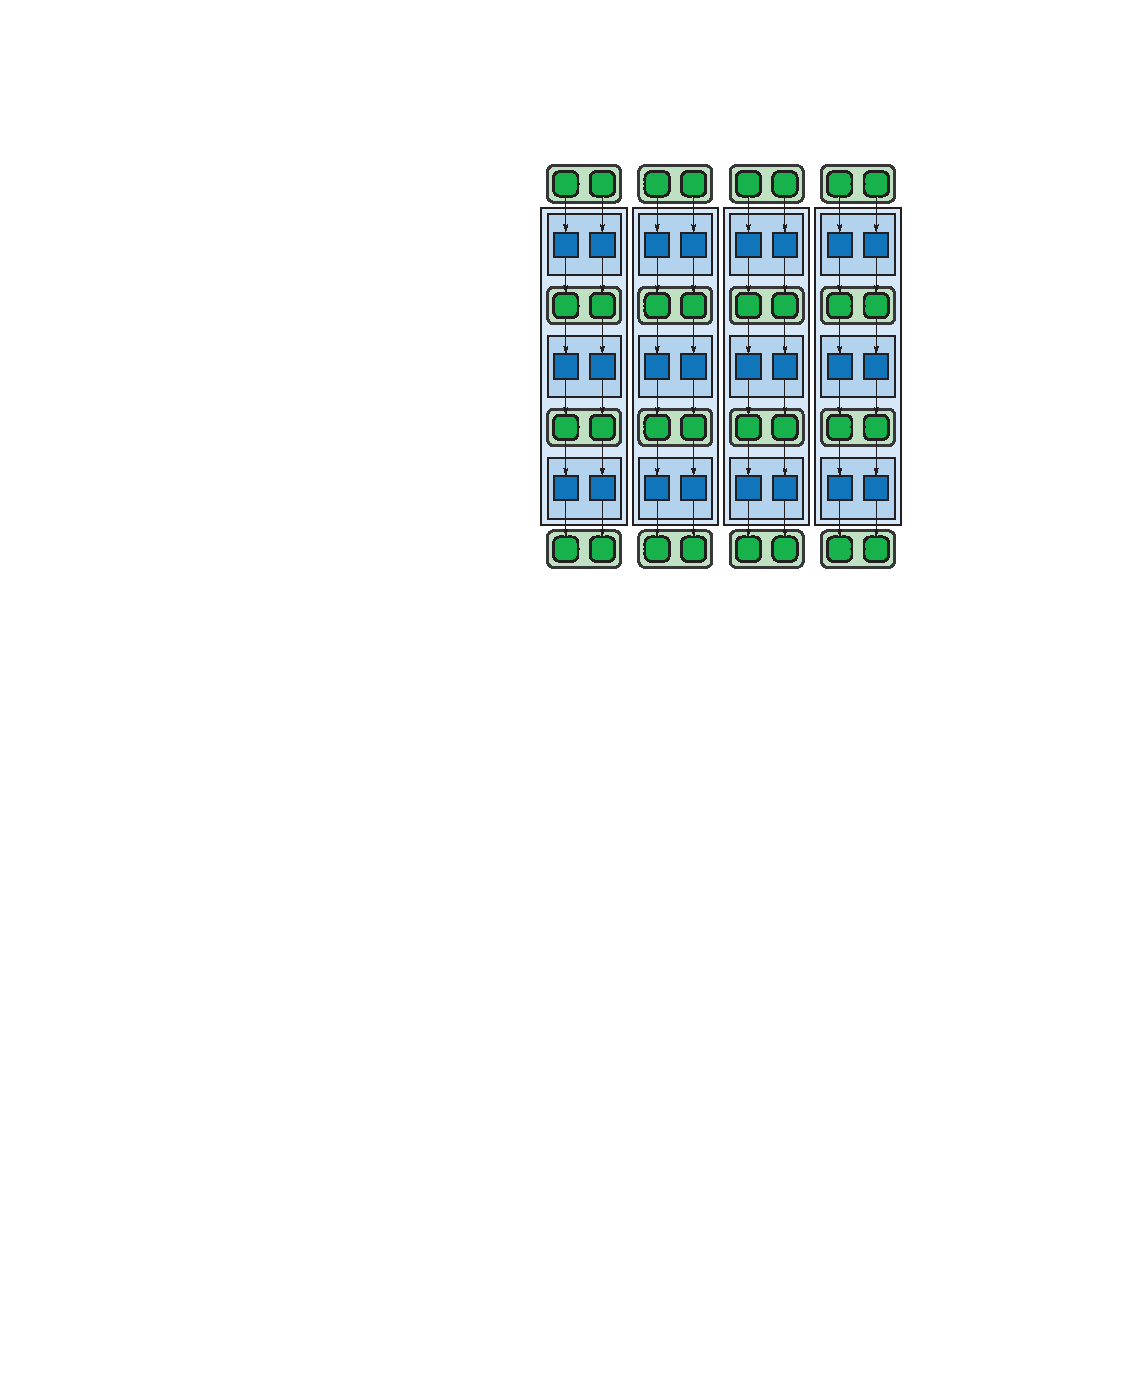
\includegraphics[width=0.9\textwidth]{images/figure-4-3-2}
	        	\end{column}
      		\end{columns}
		\end{frame}
%-----------------------------------------------------------------------------%
% End: Optimizations
%-----------------------------------------------------------------------------%


%=============================================================================%
% Section -> Related Patterns
%=============================================================================%
\section{Related Patterns} 

	\begin{frame} \frametitle{Table of Contents}
		%\tableofcontents
		%\tableofcontents[pausesections]
		\tableofcontents[currentsection]
	\end{frame} 
	
	\subsection*{Overview}
        \begin{frame} \frametitle{Overview}
            There are several patterns related to map. Three are discussed here:
            stencil, workpile, and divide-and-conquer. They will be discussed 
            more in detail in a later lecture. Remember maps apply when you can 
            perform the same operation on multiple elements with no dependencies.
        \end{frame}
	
	\subsection*{Related Patterns}
        \begin{frame} \frametitle{Stencil}
            \begin{itemize}
                \item Each instance of the map function accesses neighbors of 
                its input, offset from its usual input
                \item Common in imaging and PDE solvers
            \end{itemize}
        \end{frame}
        
		\begin{frame} \frametitle{Workpile}
			\begin{itemize}
				\item Work items can be added to the map while it is in 
                progress, from inside map function instances
				\item Work grows and is consumed by the map
				\item Workpile pattern terminates when no more work is
                available 
			\end{itemize}
	
		\end{frame}
		
		\begin{frame}[fragile] \frametitle{Divide-and-Conquer}
			\begin{itemize}
				\item Applies if a problem can be divided into smaller 
                subproblems recursively until a base case is reached that can
                be solved serially
			\end{itemize}
				\begin{verbatim}
					void DivideAndConquer( Problem P ) {
					   if ( P is base case ) {
					      Solve P;
					   } else {
					      Divide P into K subproblems;
					      Fork to conquer each subproblem in parallel;
					      Join;
					      Combine subsolutions into final solution;
					   }
					}
				\end{verbatim}
		\end{frame}
%-----------------------------------------------------------------------------%
% End: Related Patterns
%-----------------------------------------------------------------------------%



\end{document}
%END ALL

